\documentclass[10pt,a4paper]{article}
\usepackage{amsmath}
\usepackage{amssymb}
\usepackage{graphicx}
\usepackage{color}
\usepackage{fancyhdr}
\usepackage{fancyvrb}
\usepackage[margin=3.5cm]{geometry}
\usepackage{framed}
\usepackage{enumerate}
\usepackage{textcomp}
\def\ket#1{\left|#1\right\rangle}
\def\bra#1{\left\langle#1\right|}
\def\braket#1{\left\langle#1\right\rangle}

\definecolor{linkcol}{rgb}{0.0, 0.0, 0.5}
\usepackage[colorlinks=true,urlcolor=linkcol,citecolor=black,linkcolor=linkcol]{hyperref}

\renewcommand\thesection{3.\arabic{section}}
\renewcommand\thesubsection{\thesection.\arabic{subsection}}

\fancyhf{}
\lhead{\tiny Y.~D.~Chong (2016)}
\rhead{\scriptsize MH2801: Complex Methods for the Sciences}
\lfoot{}
\rfoot{\thepage}
\pagestyle{fancy}

\makeatletter
\def\PY@reset{\let\PY@it=\relax \let\PY@bf=\relax%
    \let\PY@ul=\relax \let\PY@tc=\relax%
    \let\PY@bc=\relax \let\PY@ff=\relax}
\def\PY@tok#1{\csname PY@tok@#1\endcsname}
\def\PY@toks#1+{\ifx\relax#1\empty\else%
    \PY@tok{#1}\expandafter\PY@toks\fi}
\def\PY@do#1{\PY@bc{\PY@tc{\PY@ul
\def\PYZdl{\char`\$}
\def\PYZhy{\char`\-}
\def\PYZsq{\char`\'}
\def\PYZdq{\char`\"}
\def\PYZti{\char`\~}

\begin{document}
\setcounter{page}{18}
\noindent
\underline{\textbf{\LARGE 3. Complex Numbers}}
\vskip 0.1in

The \textbf{imaginary unit}, denoted $i$, is a hypothetical solution
to the quadratic equation
\begin{equation}
z^2 + 1 = 0,
\end{equation}
which is an equation that lacks real solutions. In other words, $i =
\sqrt{-1}$.

We can let the imaginary unit take part in the usual arithmetic
operations of addition and multiplication, treating it as an algebraic
quantity on the same footing as the more familiar real numbers. Thus,
we deal with numbers containing both real and imaginary parts, called
\textbf{complex numbers}. It is one of the most profound discoveries
of mathematics that this seemingly arbitrary idea gives rise to
powerful computational methods for addressing mathematical and
physical problems.

\section{Complex algebra}
\label{complex-algebra}

For any complex number $z$, we can write
\begin{equation}
  z = x + i y,
\end{equation}
where $x$ and $y$ are real numbers that depend uniquely on $z$. We
refer to these as the \textbf{real part} of $z$ and the
\textbf{imaginary part} of $z$, respectively.  The real and imaginary
parts are also commonly denoted as $\mathrm{Re}(z)$ and
$\mathrm{Im}(z)$, respectively, where the $\mathrm{Re}$ and
$\mathrm{Im}$ operations can be regarded as functions mapping complex
numbers to real numbers

The set of complex numbers is denoted by $\mathbb{C}$. We can define
algebraic operations on complex numbers---addition/subtraction,
products, and taking powers---simply by following the usual rules of
algebra and setting $i^2 = -1$ whenever it shows up.

\begin{framed}
\noindent
\underline{\textbf{Example}}
\vskip 0.1in \noindent
Let $z = x + i y$, where $x, y \in \mathbb{R}$. What is
$z^2$?
\begin{align}
  z^2 &= (x+iy)^2 \\
  &= x^2 + 2x(iy) + (iy)^2 \\
  &= x^2 - y^2 + 2ixy
\end{align}
Therefore, the real and imaginary parts are:
\begin{equation}
\mathrm{Re}(z^2) = x^2 -y^2, \;\;\; \mathrm{Im}(z^2) = 2xy.
\end{equation}
\end{framed}

There's one caveat: for now, we'll only consider taking \emph{integer}
powers, such as $z^{-1}$ or $z^2$. Taking non-integer powers, such as
$z^{1/3}$, introduces vexatious complications which we'll postpone for
now (this will be dealt with when discussing branch points and branch
cuts).

Another interesting fact, which can be easily proven, is that real
coefficients can be freely moved into or out of $\textrm{Re}(\cdots)$
and $\textrm{Im}(\cdots)$ operations:
\begin{equation}
\left\{\begin{array}{l}\mathrm{Re}(\alpha z + \beta z') = \alpha \, \mathrm{Re}(z) + \beta\, \mathrm{Re}(z')\\ \mathrm{Im}(\alpha z + \beta z') = \alpha \, \mathrm{Im}(z) + \beta\, \mathrm{Im}(z')\end{array}\right.\qquad\mathrm{for}\;\alpha, \beta \in \mathbb{R}.
\end{equation}
This has an important consequence: if we have a complex function of a
real variable, then we can calculate the derivative of that function
from the derivatives of the real and imaginary parts.  This is shown
in the example below.

\begin{framed}
\noindent
\underline{\textbf{Example}}
\vskip 0.1in \noindent
If $z(t)$ is a complex function of a real input $t$, then
\begin{equation}
  \mathrm{Re}\left[\frac{dz}{dt}\right] = \frac{d}{dt} \mathrm{Re}\left[z(t)\right], \;\;\textrm{and}\;\;\; \mathrm{Im}\left[\frac{dz}{dt}\right] = \frac{d}{dt} \mathrm{Im}\left[z(t)\right].
\end{equation}
This can be proven using the definition of the derivative:
\begin{align*}
  \mathrm{Re}\left[\frac{dz}{dt}\right] &= \;\; \mathrm{Re}\left[\lim_{\delta t \rightarrow 0} \frac{z(t+\delta t) - z(t)}{\delta t}\right] \\
  &= \lim_{\delta t \rightarrow 0} \left[\frac{\mathrm{Re}[z(t+\delta t)] - \mathrm{Re}[z(t)]}{\delta t}\right] \\
  &= \frac{d}{dt} \mathrm{Re}\left[z(t)\right].
\end{align*}
The $\mathrm{Im}$ case works out similarly. Note that the
infinitesimal quantity $\delta t$ is real; otherwise, this wouldn't
work.
\end{framed}

\section{Conjugates and Magnitudes}\label{magnitudes-and-conjugates}

For each complex number $z = x + iy$, we define its \textbf{complex
  conjugate} as a complex number whose imaginary part has its sign
flipped:
\begin{equation}
  z^* = x - i y.
\end{equation}
We can show that conjugation obeys two important properties:
\begin{align}
  (z_1 + z_2)^* &= z_1^* + z_2^* \\
  (z_1 z_2)^* &= z_1^* z_2^*.
\end{align}

\begin{framed}
\noindent
\underline{\textbf{Example}}
\vskip 0.1in \noindent
Let us prove that $(z_1 z_2)^* = z_1^* z_2^*$. First, let
$z_1 = x_1 + i y_1$ and $z_2 = x_2 + i y_2$.
Then,
\begin{align*}
  (z_1 z_2)^* &= \left[(x_1+iy_1)(x_2+iy_2)\right]^* \\
  &= \left[\left(x_1 x_2 - y_1 y_2\right) + i\left(x_1y_2+y_1x_2\right)\right]^* \\
  &= \left(x_1 x_2 - y_1 y_2\right) - i\left(x_1y_2+y_1x_2\right) \\
  &= \left(x_1 - i y_1\right)\left(x_2 - i y_2\right) \\
  &= z_1^* z_2^*.
\end{align*}
\end{framed}

For a complex number $z = x + i y$, we define the \textbf{magnitude}
of $z$ as
\begin{equation}
  |z| = \sqrt{x^2 + y^2}.
\end{equation}
This is a non-negative real number.  A complex number and its
conjugate have the same magnitude: $|z| = |z^*|$.  Also, we can show
that magnitudes have the property
\begin{equation}
  |z_1 z_2| = |z_1| \, |z_2|.
\end{equation}
This property is similar to the ``absolute value'' operation for real
numbers, hence the similar notation.  As a corollary, we can show that
taking a power of a complex number raises its magnitude by the same
power:
\begin{equation}
  |z^n| = |z|^n \;\;\;\textrm{for}\;\;n \in \mathbb{Z}.
\end{equation}

\section{Euler's formula}\label{eulers-formula}

Euler's formula is an extremely important result which states that
\begin{equation}
e^{iz} = \cos(z) + i \sin(z).
\end{equation}
This can be proven using the series definition of the exponential
function, which is
\begin{equation}
  \exp(z) = 1 + z + \frac{z^2}{2!} + \frac{z^3}{3!} + \frac{z^4}{4!} + \frac{z^5}{5!} + \frac{z^6}{6!} + \cdots
\end{equation}
Previously, we assumed that the input to the exponential function was
a real number. However, since complex numbers can be added and
multiplied using the same rules of algebra as real numbers, we can
employ this series formula as the definition of the \textbf{complex
  exponential function}. This is a function that takes complex inputs
and gives complex outputs. When the input happens to be real, the
complex exponential function gives the same output as the real
exponential function.

Plugging $iz$ as the input to the complex exponential function gives
\begin{align}
  \exp(iz) &= 1 + (iz) + \frac{(iz)^2}{2!} + \frac{(iz)^3}{3!} + \frac{(iz)^4}{4!} + \frac{(iz)^5}{5!} + \frac{(iz)^6}{6!} + \cdots \\&= 1 + iz - \frac{z^2}{2!} - i \frac{z^3}{3!} + \frac{z^4}{4!} + i \frac{z^5}{5!} - \frac{z^6}{6!} + \cdots \\& = \left(1 - \frac{z^2}{2!} + \frac{z^4}{4!} - \frac{z^6}{6!} + \cdots\right) + i\left(z  - \frac{z^3}{3!}  + \frac{z^5}{5!}  - \frac{z^7}{7!} + \cdots\right).
\end{align}
Now, compare the two terms in parentheses to the series expansions for
the cosine and sine functions. We can define the \textbf{complex
  cosine} and \textbf{complex sine} functions using these complex
series formulas:
\begin{align}
  \cos(z) &= 1 - \frac{z^2}{2!} + \frac{z^4}{4!} - \frac{z^6}{6!} + \cdots \\
  \sin(z) &= z - \frac{z^3}{3!} + \frac{z^5}{5!} - \frac{z^7}{7!} + \cdots
\end{align}
These are perfect matches for the two terms in the series expansion of
the complex exponential! Hence, Euler's formula immediately follows:
\begin{equation}
  e^{iz} = \cos(z) + i \sin(z).
\end{equation}
One important consequence of Euler's formula is that
\begin{equation}
  \left|e^{i\theta}\right| = \sqrt{\cos^2(\theta) + \sin^2(\theta)}
  = 1 \qquad \mathrm{for}\; \theta \in \mathbb{R}.
\end{equation}
Another interesting consequence is that
\begin{equation}
  e^{i\pi} = -1,
\end{equation}
which is a formula that relates two transcendental constants $e =
2.7182818285\dots$ and $\pi = 3.141592654\dots$, by means of the
imaginary unit. (We saw a different relationship between these two
constants when solving the Gaussian integral.)

\section{The complex plane}\label{the-complex-plane}

A convenient device for conceptualizing complex numbers is to think of
a complex number as a point on a two-dimensional plane, as shown
below.  This is called the \textbf{complex plane}.

\begin{figure}[h]
  \centering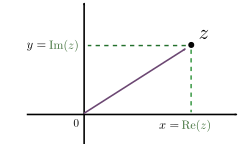
\includegraphics[width=0.32\textwidth]{complex_plane}
\end{figure}

\noindent
The real and imaginary parts are represented by horizontal and
vertical Cartesian coordinates.  The coordinate axes are called the
``real axis'' and the ``imaginary axis'', respectively.

\subsection{Polar representation}\label{polar-representation}

If we think of a complex number as a point on the complex plane, its
position can also be represented using polar coordinates instead of
Cartesian coordinates. For a complex number $z = x + i y$, we can
introduce polar coordinates $r$ and $\theta$ (both real numbers), such
that
\begin{equation}
  r = \sqrt{x^2 + y^2}, \;\;\; \theta = \tan^{-1}(y/x).
\end{equation}
Conversely,
\begin{equation}
  x = r\cos\theta, \;\;\; y = r\sin\theta.
\end{equation}
These are the usual formulas for performing a change of coordinate
between two-dimensional Cartesian coordinates and polar coordinates.
Their graphical meaning is shown below:

\begin{figure}[h]
  \centering\includegraphics[width=0.32\textwidth]{complex_plane2}
\end{figure}

\noindent
The radial coordinate is $r$, and by its definition we see that it is
equal to what we have defined as the
\hyperref[magnitudes-and-conjugates]{magnitude} of the complex number:
$r = |z|$. The azimuthal coordinate $\theta$ is called the
\textbf{argument} of the complex number, which we sometimes denote by
$\mathrm{arg}(z)$.

Using \hyperref[eulers-formula]{Euler's formula}, we can write
\begin{align}
  z &= r\cos(\theta) + i r\sin(\theta)\\
  &= r \left[\cos(\theta) + i \sin(\theta)\right] \\
  &= r \, e^{i\theta}.
\end{align}
Thus, whenever we can manipulate a complex number into a form $A
e^{iB}$, where $A$ and $B$ are real, then $A$ is the magnitude and $B$
is the argument. This is used in the following example:

\begin{framed}
\noindent
\underline{\textbf{Example}}
\vskip 0.1in \noindent
For $z \in \mathbb{C}$, it can be shown that the magnitude and argument
of $\exp(z)$ are:
\begin{equation}
  \left|\exp(z)\right| = e^{\mathrm{Re}(z)}, \quad
  \mathrm{arg}\left[\exp(z)\right] = \mathrm{Im}(z).
\end{equation}
Proof: Let $z = x + i y$, where $x, y \in \mathbb{R}$; then
\begin{equation}
  e^{z} = e^{x + i y} = e^x \, e^{iy}.
\end{equation}
By inspection, the magnitude of this complex number is $e^x$, and its
argument is $y$.
\end{framed}

\subsection{Geometrical interpretation of complex operations}
\label{geometrical-interpretation-of-complex-operations}

The complex plane provides useful geometric interpretations for
complex algebra operations:

\begin{itemize}
\item
  Addition of two complex numbers can be interpreted as the addition
  of two coordinate vectors. If $z_1 = x_1 + i y_1$ and $z_2 = x_2 + i
  y_2$, then $z_1 + z_2 = \left(x_1 + x_2\right) + i\left(y_1 +
  y_2\right).$

  Hence, the point corresponding to $z_1 + z_2$ is obtained by adding
  the two coordinate vectors corresponding to $z_1$ and $z_2$. From
  this, we can geometrically prove a useful inequality relation
  between complex numbers, called the ``triangle inequality'':
  \begin{equation}
    |z_1 + z_2| \le |z_1| + |z_2|.
  \end{equation}

\item
  Complex multiplication can be interpreted as a scaling together with
  a rotation. If $z_1 = r_1e^{i\theta_1}$ and $z_2 =
  r_2e^{i\theta_2}$, then $z_1 z_2 = \left(r_1 r_2\right)
  \,\exp[i(\theta_1 + \theta_2)]$.  The point corresponding to $z_1 \,
  z_2$ is obtained by scaling the $z_1$ coordinate vector by a factor
  of $|z_2|$, and rotating it by an angle of $\theta_2$ around the
  origin. In particular, multiplication by $e^{i\theta}$ is equivalent
  to a pure rotation of angle $\theta$.

\item
  \hyperref[magnitudes-and-conjugates]{Complex conjugation} is
  equivalent to reflection about the real axis. This moves a point
  from the ``upper half'' of the complex plane to the ``lower half'',
  or vice versa.
\end{itemize}

\section{Complex functions}\label{complex-functions}

When deriving \protect\hyperlink{euler_formula}{Euler's formula}, we
introduced \textbf{complex functions} defined by taking
\href{00_mathfunctions.ipynb}{real mathematical functions}, such as
the \href{00_mathfunctions.ipynb\#exponential}{exponential function},
and making them accept complex number inputs. Let us take a closer
look at how these complex functions behave.

\subsection{Complex trigonometric functions}
\label{complex-trigonometric-functions}

When we derived \protect\hyperlink{euler_formula}{Euler's formula}, we
noted that it is valid for arbitrary real numbers:
\begin{equation}
  \exp(iz) = \cos(z) + i \sin(z), \quad \mathrm{for}\;\;z\in\mathbb{C}.
\end{equation}
The cosine and sine functions on the right-hand side of this equation
are \textit{complex} trigonometric functions, defined using the same
series expansions as the real cosine and sine functions, except that
the inputs $z$ are allowed to be complex numbers:
\begin{align}
  \sin(z) &= z - \frac{z^3}{3!} + \frac{z^5}{5!} - \frac{z^7}{7!} + \cdots \\
  \cos(z) &= 1 - \frac{z^2}{2!} + \frac{z^4}{4!} - \frac{z^6}{6!} + \cdots, 
  \quad\quad z\in \mathbb{C}
\end{align}
Note that the outputs of the complex trigonometric functions are
complex numbers too. Thus, some of the familiar properties of the real
trigonometric functions don't apply. For instance, $|\sin(z)|$ and
$|\cos(z)|$ are \emph{not} bounded by 1 when $z$ is not real. For
example,
\begin{equation}
\Big|\sin(i)\Big| \;=\; 1.1752\dots \; >\; 1.
\end{equation}

We can also write the complex cosine and sine functions in terms of
the exponential:
\begin{align}
  \cos(z) &= \;\;\frac{1}{2}\left(e^{iz} + e^{-iz}\right) \\
  \sin(z) &= -\frac{i}{2}\left(e^{iz} - e^{-iz}\right).
\end{align}
This is often a convenient step when solving integrals, as shown in
the following example.

\begin{framed}
\noindent
\underline{\textbf{Example}}
\vskip 0.1in \noindent
Consider the (real) integral
\begin{equation}
I = \int_0^\infty dx \; e^{- x} \, \cos(x).
\end{equation}
One way to solve this is to use integration by parts, but another way
is to use the complex expansion of the cosine function:
\begin{align}I &= \int_0^\infty dx \; e^{- x} \,\frac{1}{2}\, \left[e^{ix} + e^{-ix}\right] \\ &= \frac{1}{2} \int_0^\infty dx \; \left[e^{(-1+i)x} + e^{(-1-i)x}\right] \\ &= \frac{1}{2} \left[ \frac{e^{(-1+i) x}}{-1+i} + \frac{e^{(-1 - i) x}}{-1 - i}\right]_0^\infty \\ &= -\frac{1}{2} \left(\frac{1}{-1+i} + \frac{1}{-1 - i}\right) \\ &= \frac{1}{2}.\end{align}
\end{framed}

\subsection{Complex trigonometric identities}
\label{complex-trigo}

Euler's formula provides a convenient way to deal with trigonometric
functions. Consider the addition formulas
\begin{align}
  \sin(z_1 + z_2) &= \sin(z_1) \cos(z_2) + \cos(z_1)\sin(z_2) \\
  \cos(z_1 + z_2) &= \cos(z_1) \cos(z_2) - \sin(z_1)\sin(z_2).
\end{align}
The standard proofs for these formulas are geometric: you draw a
figure, and solve a bunch of relations between the angles and sides of
the various triangles, making use of the Pythagorean formula. But
using the Euler formula, we can prove these algebraically.  For
example,
\begin{align}
  \cos(z_1)\cos(z_2) &= \frac{1}{4}\left(e^{iz_1} + e^{-iz_1}\right) \left(e^{iz_2} + e^{-iz_1}\right)\\
  &= \frac{1}{4}\left[e^{i(z_1+z_2)} + e^{i(-z_1 + z_2)} + e^{i(z_1 -z_2)} + e^{-i(z_1+z_2)}\right] \\
  \sin(z_1)\sin(z_2) &= -\frac{1}{4}\left(e^{iz_1} - e^{-iz_1}\right) \left(e^{iz_2} - e^{-iz_1}\right) \\
  &= -\frac{1}{4}\left[e^{i(z_1+z_2)} - e^{i(-z_1 + z_2)} - e^{i(z_1 -z_2)} + e^{-i(z_1+z_2)}\right].
\end{align}
Thus,
\begin{equation}
  \cos(z_1) \cos(z_2) - \sin(z_1)\sin(z_2)
  = \frac{1}{2}\left[e^{i(z_1+z_2)} + e^{-i(z_1+z_2)}\right] = \cos(z_1 + z_2).
\end{equation}
As a bonus, these addition formulas now hold for complex inputs as
well, not just real inputs. Higher-order trigonometric addition
formulas can be derived in a similar way.

\subsection{Hyperbolic functions}\label{hyperbolic-functions}

Euler's formula also provides us with a link between the trionometric
and hyperbolic functions. From the definition of the hyperbolic
functions:
\begin{equation}
\sinh(z) = \frac{1}{2}\left(e^{z} - e^{-z}\right), \quad\;
\cosh(z) = \frac{1}{2}\left(e^{z} + e^{-z}\right)
\end{equation}
Compare this to \hyperref[complex-trigo]{our above definition of the
  complex trigonometric functions}:
\begin{equation}
\sin(z) = -\frac{i}{2}\left(e^{iz} - e^{-iz}\right), \;\;\; \cos(z) = \;\;\frac{1}{2}\left(e^{iz} + e^{-iz}\right)
\end{equation}
From this, we can see that the trigonometric and hyperbolic functions
are related by
\begin{align}
\sin(z) &= -i \sinh(iz), \quad \cos(z) = \cosh(iz) \\
\sinh(z) &= -i \sin(iz), \quad \cosh(z) = \cos(iz)
\end{align}
Using these relations, we can relate the addition formulas for
trignometric formulas to the addition formulas for hyperbolic
functions, e.g.
\begin{align}
  \cosh(z_1+z_2) &= \cos(iz_1 + iz_2) \\
  &= \cos(iz_1)\cos(iz_2) - \sin(iz_1)\sin(iz_2) \\
  &= \cosh(z_1)\cosh(z_2) + \sinh(z_1)\sinh(z_2).
\end{align}

\section{Trajectories in the complex plane}
\label{trajectories-in-the-complex-plane}

If we have a function $z(t)$ that takes a real input $t$ and gives a
complex output $z$, it is often useful to plot a curve in the complex
plane, called the ``parametric trajectory'' of $z$. Each point on the
curve gives the value of $z$ at some $t$. We will give a few examples
below.

First, consider
\begin{equation}
  z(t) = e^{i\omega t}, \quad \omega \in \mathbb{R}.
\end{equation}
The trajectory is a circle in the complex plane, centered at the
origin and with radius 1:

\begin{figure}[h]
  \centering\includegraphics[width=0.37\textwidth]{complex_trajectory_1}
\end{figure}

\noindent
To see why, observe that the function has the form $z(t) =
r(t)\,e^{i\theta(t)}$, where the magnitude (i.e., the distance from
the origin) $r(t) = 1$ is a constant, and the argument $\theta(t) =
\omega t$ varies proportionally with $t$. If $\omega$ is positive, the
argument increases with $t$, so the trajectory is counter-clockwise,
as shown in the above figure. If $\omega$ is negative, the trajectory
is clockwise.

Next, consider
\begin{equation}
  z(t) = e^{(\gamma + i \omega) t}, \;\;\;\mathrm{where}\;\;
  \gamma,\omega \in \mathbb{R}.
\end{equation}
For $\gamma = 0$, this reduces to the previous example. For $\gamma
\ne 0$, the trajectory is a spiral:

{\centering
\includegraphics[width=0.37\textwidth]{complex_trajectory_2}\par
}

\noindent
To see why, observe that this function can be written in the form
\begin{equation}
  z(t) = r(t) \;e^{i\theta(t)},
\end{equation}
where $r(t) = e^{\gamma t}$ and $\theta = \omega t.$ Similar to the
previous example, the argument varies proportionally with $t$, so the
trajectory loops around the origin. What's different is that the
magnitude (i.e., the distance from the origin) now either increases or
decreases exponentially with $t$, depending on the sign of $\gamma$.
If $\gamma$ and $\omega$ are both positive, then the trajectory is
an anticlockwise spiral moving outwards from the origin. You should work
out for yourself how and why the trajectory behaves if we flip the signs
of $\gamma$ and/or $\omega$.
    
Finally, consider
\begin{equation}
  z(t) = \frac{1}{\alpha t + \beta}, \quad \alpha,\beta \in \mathbb{R}.
\end{equation}
This trajectory is a circle which passes through the origin, as shown
below:

\begin{figure}[h]
  \centering\includegraphics[width=0.37\textwidth]{complex_trajectory_3}
\end{figure}

\noindent
The proof is left as an exercise. This is something called a
\href{http://en.wikipedia.org/wiki/M\%C3\%B6bius_transformation}{M\"obius
  transformation}.

\section{Why complex numbers? (Optional)}\label{why-complex-numbers-optional}

You may wonder what makes the square root of $-1$ an interesting
mathematical object, such that it's used to define a whole new system
of ``complex numbers''. You may also wonder whether complex numbers
are the only generalization of real numbers; could the concept be
usefully extended to even more complicated number systems?

To answer these questions, we observe that complex numbers can be
manipulated using the same rules of algebra as real numbers. We can
add, subtract, multiply, and divide (apart from division by zero)
complex numbers, without running into any inconsistencies.

The set of complex numbers $\mathbb{C}$ has a special property: it is
\emph{algebraically closed}, meaning that every complex polynomial
equation has solution(s) in $\mathbb{C}$. The set of real numbers,
$\mathbb{R}$, lacks this property, since equations like $x^2 + 1 = 0$
have no solution in $\mathbb{R}$. The ``closure'' property of
$\mathbb{C}$ is so important that it's called the
\href{https://en.wikipedia.org/wiki/Fundamental_theorem_of_algebra}{Fundamental
  Theorem of Algebra}. The Fundamental Theorem implies that
$\mathbb{C}$ can't be ``algebraically extended'' into a more
complicated number system the way we extended $\mathbb{R}$ into
$\mathbb{C}$.

There do exist extensions of complex numbers that discard one or more of
the rules of algebra. The
\href{https://en.wikipedia.org/wiki/Quaternion}{quaternions} are a kind
of number system where each quaternionic number has four real
components; these obey a non-commutative algebra where, generally,
$ab \ne ba$. \href{https://en.wikipedia.org/wiki/Octonion}{Octonions}
are eight-component numbers which are both non-commutative and
non-associative: $(ab)c \ne a(bc)$. These and other
still-more-complicated number systems have some applications in physics
and other fields, but are overall much less important than
$\mathbb{C}$.

Another reason complex numbers are so mathematically rich is that you
can do calculus on them. The study of smooth complex functions is
called \textbf{complex analysis}, which will be discussed later. As we
shall see, it is possible to extend the concepts of differentiation
and integration from real functions to complex functions, with many
profound outcomes. By contrast, because quaternions are not
commutative, even the concept of ``derivative'' becomes tricky to
define. Thus, it's a lot harder to perform mathematical analysis on
quaternions and other more complicated number systems.

\section{Exercises}

\begin{enumerate}
\item
  Let $z = x + iy$, where $x, y \in \mathbb{R}$. For each of the
  following expressions, find (i) the real part, (ii) the imaginary
  part, (iii) the magnitude, and (iv) the complex argument, in terms
  of $x$ and $y$:
  \begin{itemize}
  \item $z^2$
  \item $1/z$
  \item $\exp(z)$
  \item $\exp(iz)$
  \item $\cos(z)$
  \end{itemize}

\item
Show that $|z_1 z_2| = |z_1|\, |z_2|$, by using (i) the polar
representation, and (ii) the Cartesian representation.

\item
  Show that $(z_1 z_2)^* = z_1^* z_2^*$, by using (i) the polar
  representation, and (ii) the Cartesian representation.

\item
  Identify the problem with this chain of equations:
  \begin{equation*}
    -1 = i \cdot i =
    \sqrt{-1}\,\sqrt{-1} = \sqrt{-1 \cdot -1} = \sqrt{1} = 1.    
  \end{equation*}

\item
  With the aid of Euler's formula, prove that
  \begin{align}
    \cos(3x) &= 4[\cos(x)]^3 -3\cos(x)\\
    \sin(3x) &= 3\sin(x)-4[\sin(x)]^3.
  \end{align}

\item
  For $z_1, z_2 \in \mathbb{C}$ and $\theta \in \mathbb{R}$, show that
  $\mathrm{Re}\left[z_1 e^{i\theta} + z_2 e^{-i\theta}\right] = A
  \cos(\theta) + B \sin(\theta)$, for some $A, B \in \mathbb{R}$. Find
  explicit expressions for $A$ and $B$ in terms of $z_1$ and $z_2$.

\item
  In the \hyperref[the-complex-plane]{complex plane}, the conjugation
  operation corresponds to a reflection about the real axis. What
  operation corresponds to a reflection about the imaginary axis?

\item
  Consider the complex function of a real variable $z(t) = 1/(\alpha t
  + \beta)$, where $\alpha, \beta \in \mathbb{C}$ and $t \in
  \mathbb{R}$.  For $\alpha = 1$ and $\beta = i$, show that $z(t)$ can
  be re-expressed as $z(s) = (1+e^{is})/(2i)$, where $s \in
  (-\pi,\pi)$.  Hint: find a real mapping $t(s)$.

  Hence, show that the trajectory for arbitrary $\alpha,\, \beta \in
  \mathbb{C}$ forms a circle.

\item
  With the help of a computer plotting program, generate complex
  trajectories for the following functions (for real inputs $t
  \in\mathbb{R}$). Explain their key features, including the
  directions of the trajectories:
  \begin{itemize}
  \item
    $z(t) = \left[1+\frac{\cos(\beta t)}{2}\right] \, \exp(it)$, for
$\beta = 10$ and for $\beta = \sqrt{5}$.
  \item
$z(t) = -it \pm \sqrt{1 - t^2}$.
    \item
$z(t) = ae^{it} + be^{-it}$, for $a = 1, b = -2$ and for
$a = 1, b = 2$.
  \end{itemize}
\end{enumerate}
\end{document}
